% !TeX document-id = {a90a2b0a-e08e-44ed-850a-35793bedbf3a}
% !TeX TS-program = xelatex

% !BIB program = biber
\documentclass[handout]{beamer}
%\documentclass[compress]{beamer}
\usepackage[T1]{fontenc}
\usepackage{pifont}
\usetheme[block=fill,subsectionpage=progressbar,sectionpage=progressbar]{metropolis} 


\definecolor{Purple}{HTML}{911146}
\definecolor{Orange}{HTML}{CF4A30}

% Theme colors are derived from these two elements
\setbeamercolor{alerted text}{fg=Orange}

% ... however you can of course override styles of all elements
\setbeamercolor{frametitle}{bg=Purple}


\usepackage{wasysym}
\usepackage{etoolbox}
\usepackage[utf8]{inputenc}

\usepackage{threeparttable}
\usepackage{subcaption}

\usepackage{tikz-qtree}
\setbeamercovered{still covered={\opaqueness<1->{5}},again covered={\opaqueness<1->{100}}}


\usepackage{listings}

\lstset{
	basicstyle=\scriptsize\ttfamily,
	columns=flexible,
	breaklines=true,
	numbers=left,
	%stepsize=1,
	numberstyle=\tiny,
	backgroundcolor=\color[rgb]{0.85,0.90,1}
}



\lstnewenvironment{lstlistingoutput}{\lstset{basicstyle=\footnotesize\ttfamily,
		columns=flexible,
		breaklines=true,
		numbers=left,
		%stepsize=1,
		numberstyle=\tiny,
		backgroundcolor=\color[rgb]{.7,.7,.7}}}{}


\lstnewenvironment{lstlistingoutputtiny}{\lstset{basicstyle=\tiny\ttfamily,
		columns=flexible,
		breaklines=true,
		numbers=left,
		%stepsize=1,
		numberstyle=\tiny,
		backgroundcolor=\color[rgb]{.7,.7,.7}}}{}


\usepackage[american]{babel}
\usepackage{csquotes}
\usepackage[style=apa, backend = biber]{biblatex}
\DeclareLanguageMapping{american}{american-UoN}
\addbibresource{../literature.bib}
\renewcommand*{\bibfont}{\tiny}

\usepackage{tikz}
\usetikzlibrary{shapes,arrows,matrix}
\usepackage{multicol}

\usepackage{subcaption}

\usepackage{booktabs}
\usepackage{graphicx}

\graphicspath{{../pictures/}}

\makeatletter
\setbeamertemplate{headline}{%
	\begin{beamercolorbox}[colsep=1.5pt]{upper separation line head}
	\end{beamercolorbox}
	\begin{beamercolorbox}{section in head/foot}
		\vskip2pt\insertnavigation{\paperwidth}\vskip2pt
	\end{beamercolorbox}%
	\begin{beamercolorbox}[colsep=1.5pt]{lower separation line head}
	\end{beamercolorbox}
}
\makeatother



\setbeamercolor{section in head/foot}{fg=normal text.bg, bg=structure.fg}



\newcommand{\question}[1]{
	\begin{frame}[plain]
		\begin{columns}
			\column{.3\textwidth}
			\makebox[\columnwidth]{
				
\includegraphics[width=\columnwidth,height=\paperheight,keepaspectratio]{../pictures/mannetje.png}}
			\column{.7\textwidth}
			\large
			\textcolor{orange}{\textbf{\emph{#1}}}
		\end{columns}
\end{frame}}

\newcommand{\instruction}[1]{\emph{\textcolor{gray}{[#1]}}}


\title[Computational Communication Science 2]{\textbf{Computational Communication Science 2} \\Week 8 - Lecture\\ »A Deep Dive into Supervised Machine Learning«}
\author[Marthe Möller, Anne Kroon]{Marthe Möller \\ Anne Kroon \\ ~ \\ \footnotesize{a.m.moller@uva.nl, @marthemoller \\a.c.kroon@uva.nl, @annekroon} \\}
\date{May, 2022}
\institute[Digital Society Minor, University of Amsterdam]{Digital Society Minor, University of Amsterdam}


\begin{document}
	
	\begin{frame}{}
		\titlepage
\end{frame}
	
\begin{frame}{Today}
		\tableofcontents
\end{frame}


\section{Recap}

\begin{frame}{Recap}
	
	Short recap of last week.

	
\end{frame}



\section{Some classical ML models}

\begin{frame}{Regression}
	
	\begin{center}
		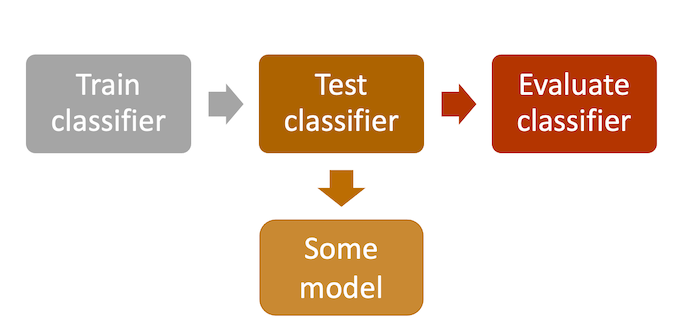
\includegraphics[width=\linewidth,height=\textheight,keepaspectratio]{../pictures/MLprocess_model.png} \\\
	\end{center}
	
	
	% When we train a model, we can do so based on different functions. Any function can be used, as long as it uses features of cases as an input and produces a prediction based on these. 
	
\end{frame}


\begin{frame}{Regression}
	
	\begin{center}
		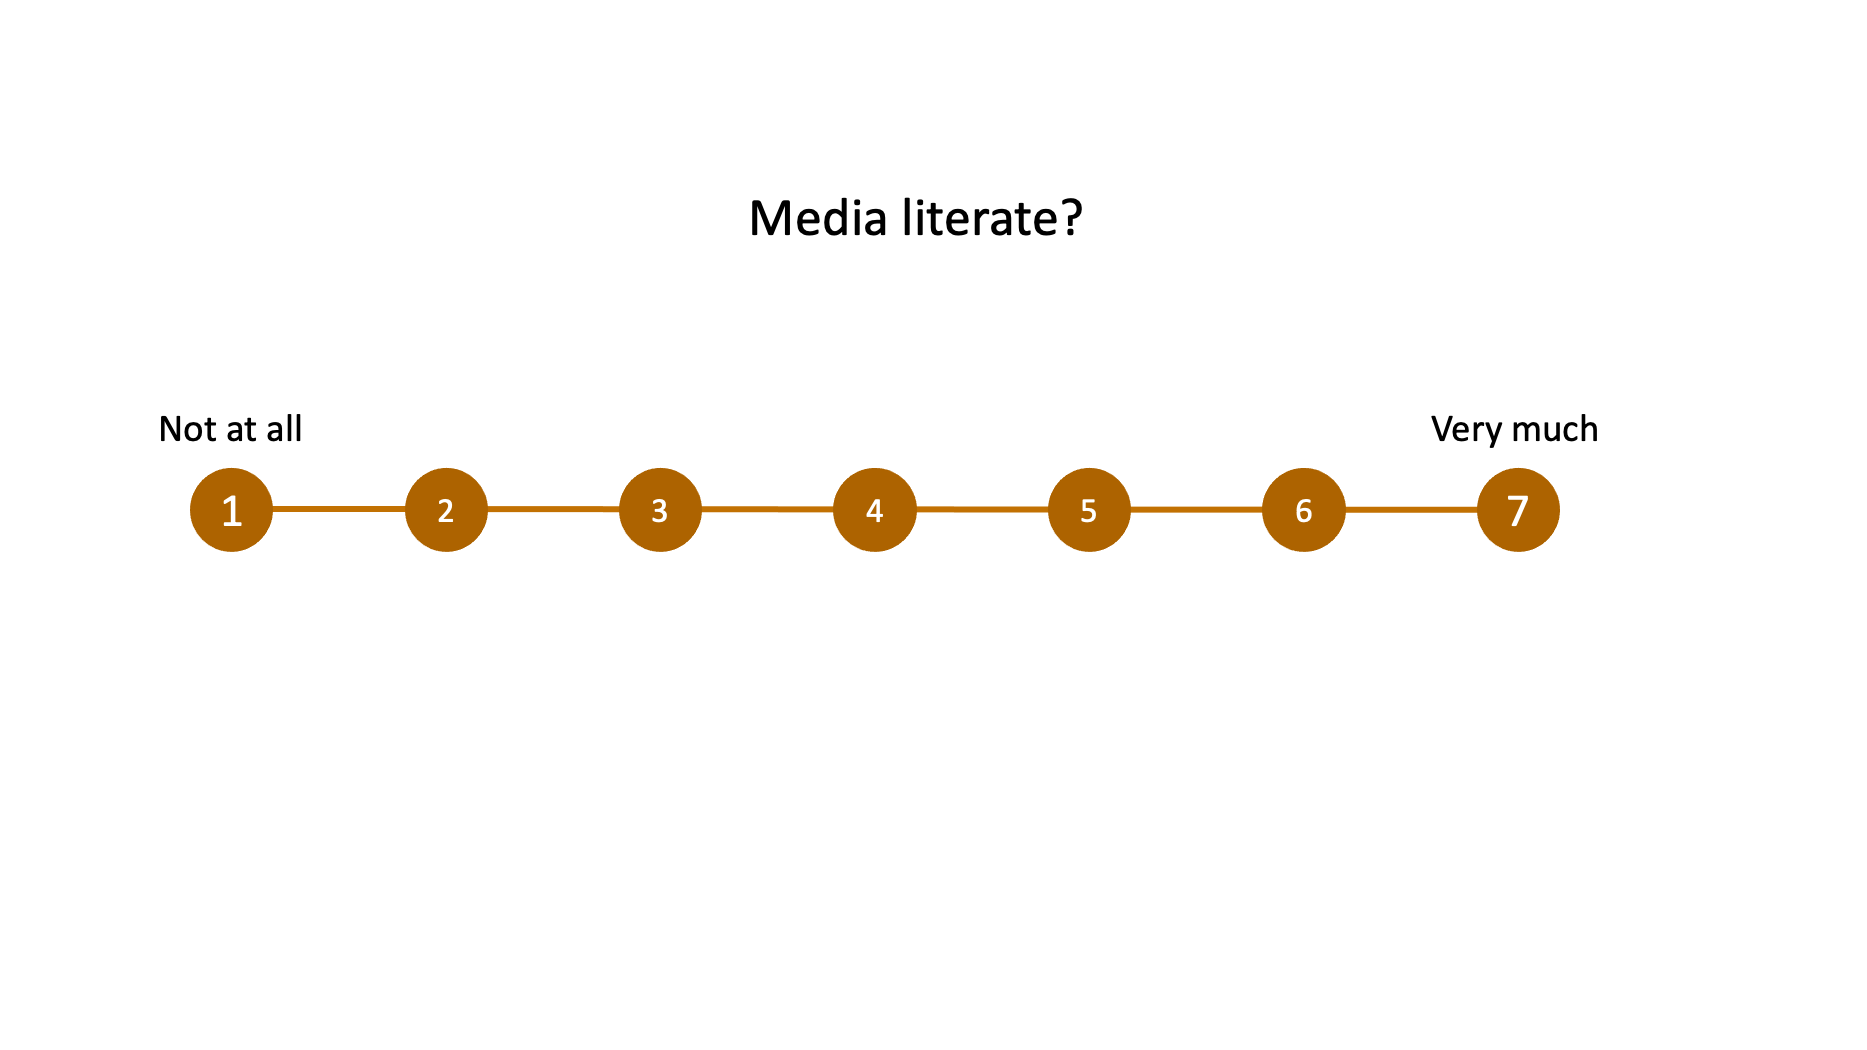
\includegraphics[width=\linewidth,height=\textheight,keepaspectratio]{../pictures/medialiteracyscale.png} \\\
	\end{center}
	
	
	% One model that can be used, is the ordinary least squares (OLS) regression model, like we just discussed.
	
	% You know from statistics courses that OLS regression predicts a case’s value on a dependent variable. For example, we use the scores of a case on two independent variables (say age and education level) to predict that persons score on a dependent variable: say, media literacy score ranging from 1 to 7.
	
	% Applying this to ML, we use the regression to predict the scores of many many cases on the DV. 
	
	
\end{frame}



\begin{frame}{Regression}
	
	\begin{center}
		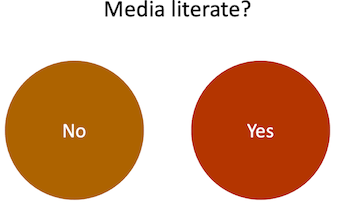
\includegraphics{../pictures/medialiteracydummy.png} \\\
	\end{center}
	
	
	% But in applications of ML, we are often not so much interested in predicting a specific value of the DV. Rather, we are interested in predicting categories. For example, based on some features, we want to predict if someone uses Instagram or not.
	
	% To predict nominal outcomes (such as Instagram user, yes or no), we use logistic regression.
	
	
\end{frame}


\begin{frame}{Regression}
	
	\begin{center}
		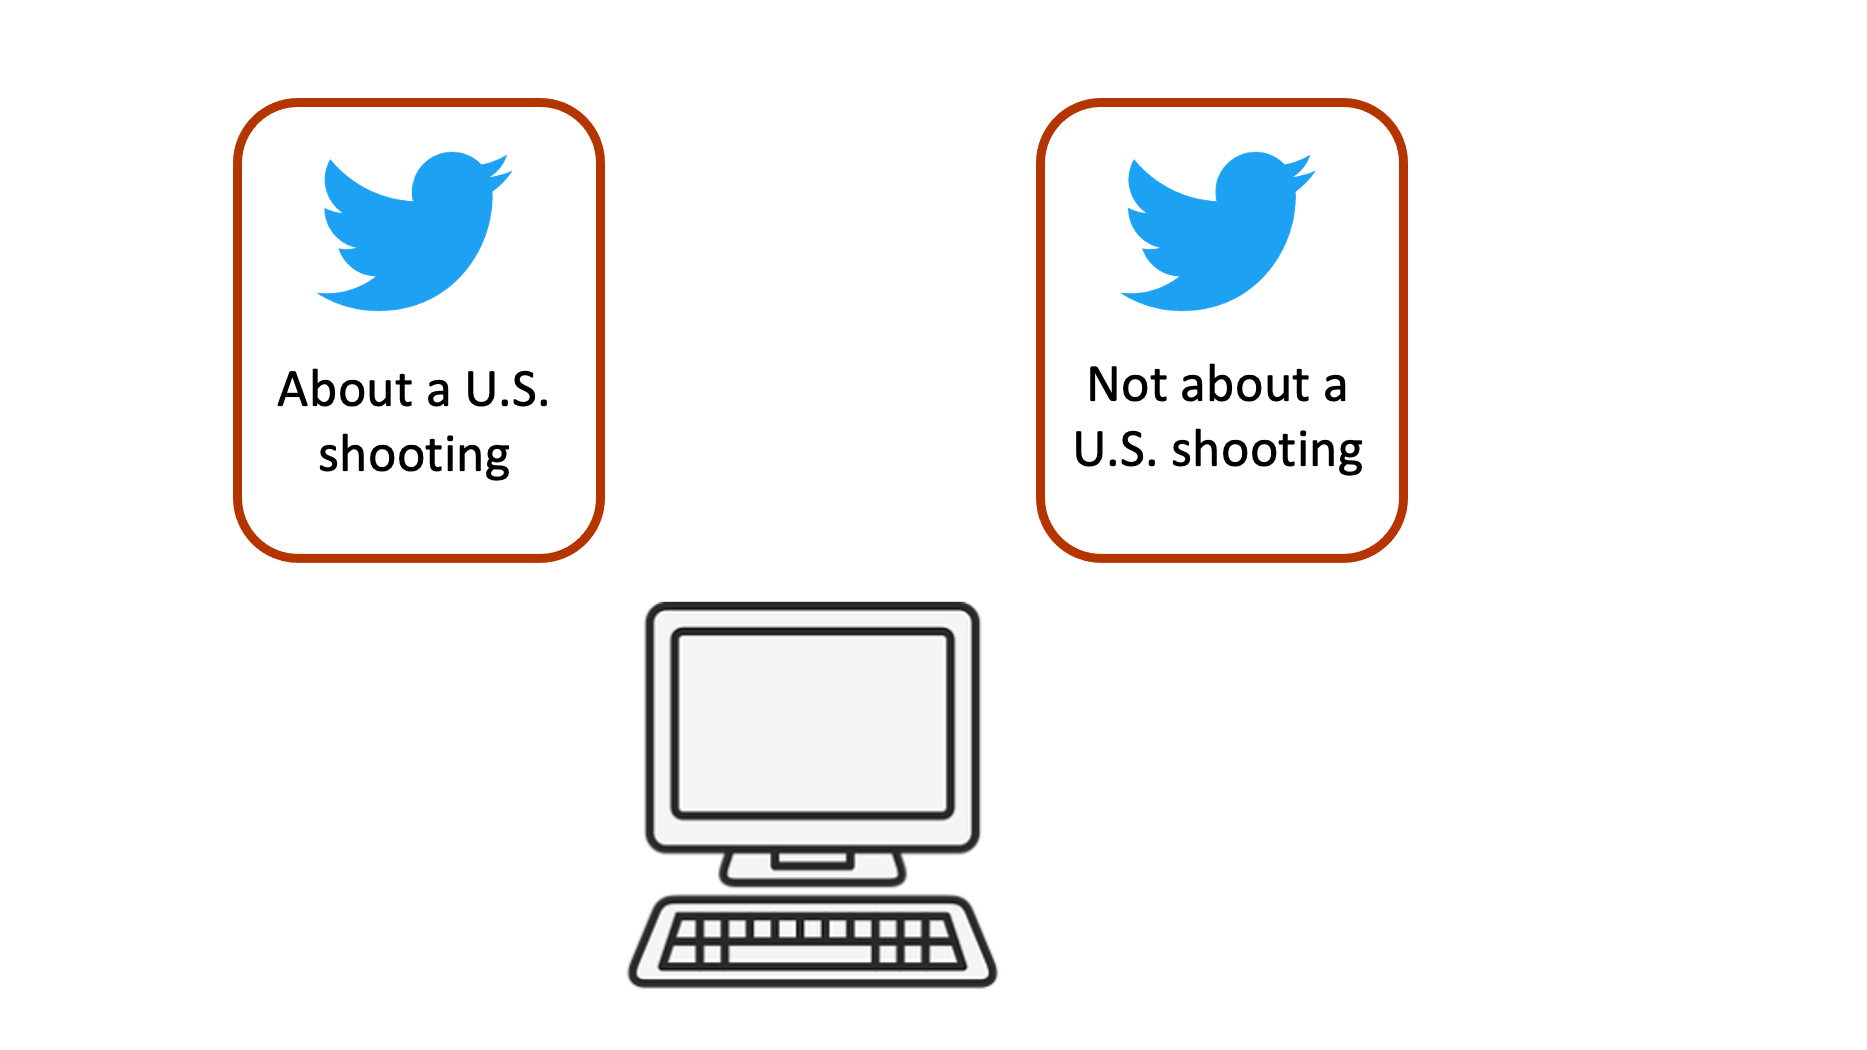
\includegraphics{../pictures/Zhangetal_1.png} \\\
	\end{center}
	
	\begin{tiny}
	\fullcite{zhang_whose_2019} 
	\end{tiny}

	% Using logistic regression in SML, it is possible to assign a category to millions of cases. How can this be used to study communication?
	
	% Example: Zhang et al. used it to analyze how people use Twitter to express grief after mass shootings. They trained a model to distinguish Tweets that were about U.S. shootings from Tweets that weren’t (two categories).
		
\end{frame}


\begin{frame}{Regression}
	
	\begin{center}
		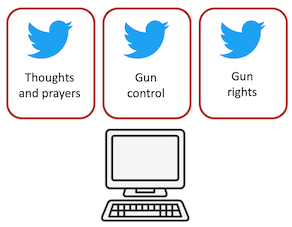
\includegraphics{../pictures/Zhangetal_2.png} \\\
	\end{center}

	\begin{tiny}
	\fullcite{zhang_whose_2019} 
	\end{tiny}
	
	% After that, they trained another model to classify relevant Tweets according to their topic in a more precise manner. Namely, the computer learned to indicate whether a Tweet was about “thoughts and prayers”, gun control or gun rights.
	
\end{frame}


\begin{frame}{Regression}
	
	\begin{center}
		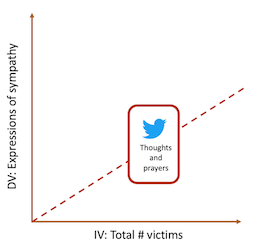
\includegraphics{../pictures/Zhangetal_3.png} \\\
	\end{center}

	\begin{tiny}
	\fullcite{zhang_whose_2019} 
	\end{tiny}
	
	
	% They then used these labels as the dependent variable in their analyses. The independent variables were (a) the total number of victims of a shooting and (b) the number of children killed. They found that mass shooting events involving both more total victims and more children killed generated more expressions of sympathy.
	
	% They also found that shootings with more African-America deaths or that are perpetrated by white shooters were related to fewer defenses of gun rights and calls for gun control…
		
\end{frame}


\begin{frame}{Na\"{\i}ve Bayes}
	
	\begin{center}
		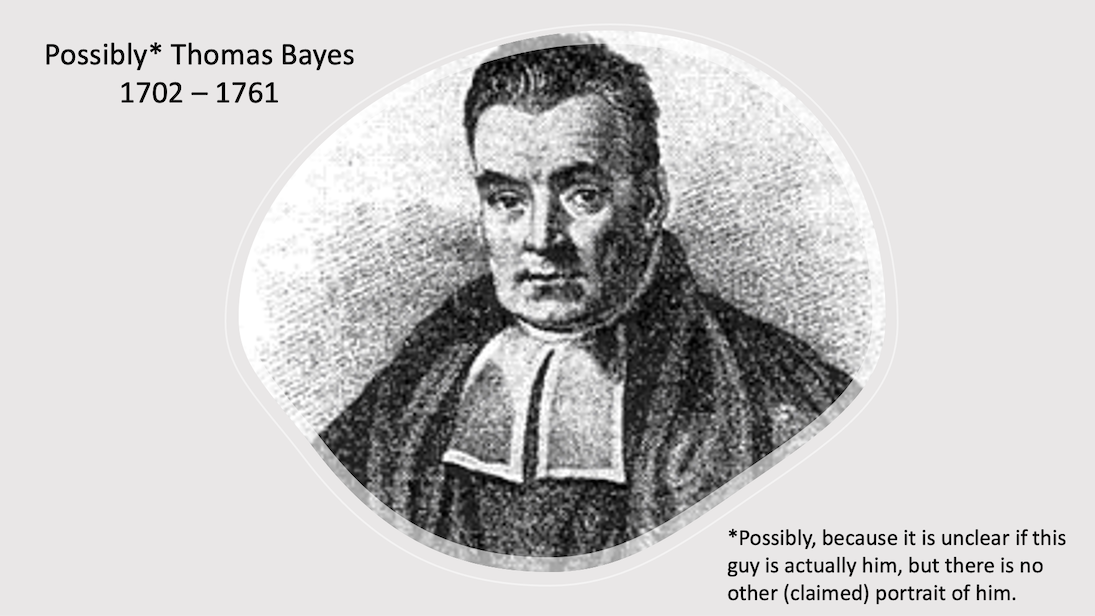
\includegraphics[width=\linewidth,height=\textheight,keepaspectratio]{../pictures/ThomasBayes.png} \\\
	\end{center}

	% Another way to predict a category is by using the Naïve Bayes classifier. Bayes because: It uses the theorem developed by Thomas Bayes. 
	
	% Naïve because: it assumes that all features are independent from each other. This is naïve because it is hardly ever the case. Think about survey data: one’s score on IV income is surely related to one’s score on IV education level. 
	
	% Although the assumptions of the Naïve Bayes classifier are often violated, it works remarkably well in practice. 
	
\end{frame}



\begin{frame}{Na\"{\i}ve Bayes}
		
	$ P(\rm{A} \mid \rm{B}) = \frac{P(\rm{B} \mid \rm{A}) \cdot P(\rm{A})}{P(\rm{B})} $

	Mathematicians’ language for: the probability of A is B is the case/present/true. 

	$ P(\rm{label} \mid \rm{features}) = \frac{P(\rm{features} \mid \rm{label}) \cdot P(\rm{label})}{P(\rm{features})} $

	
	% In our case it means: the probability of an item having a label, given a set of features. 
	
	% We use this formula to (1) train our model, (2) test it, and finally (3) evaluate our model.
	
	% Geef voorbeeld, een van de assigned readings
	
\end{frame}


\begin{frame}{Support Vector Machines}
	
	SVMs aim to find a hyperplane in an \(N\)-dimensional pace that distinctly classifies the datapoints.
	
	The best hyperplane is the one that has the maximum margin (distance) between the datapoints of both classes.
	
	\begin{center}
		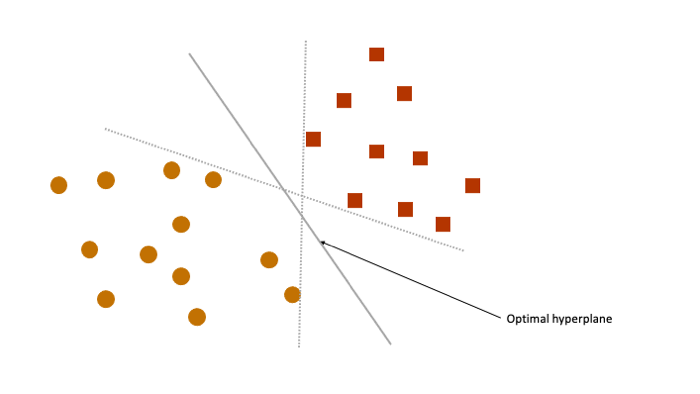
\includegraphics[width=\linewidth,height=0.5\textheight,keepaspectratio]{../pictures/optimal_hyperplane.png} \\\
	\end{center}
	
\end{frame}

\begin{frame}{Support Vector Machines}
	
	\begin{center}
		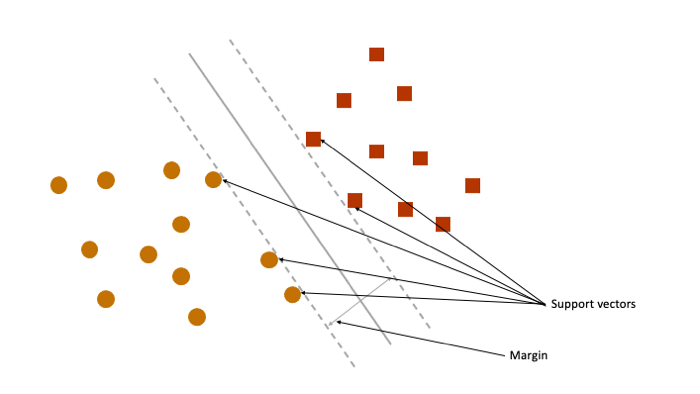
\includegraphics[width=\linewidth,height=\textheight,keepaspectratio]{../pictures/SVM.png} \\\
	\end{center}
	
\end{frame}


\begin{frame}{Decision Trees and Random Forests}
	
	\begin{center}
		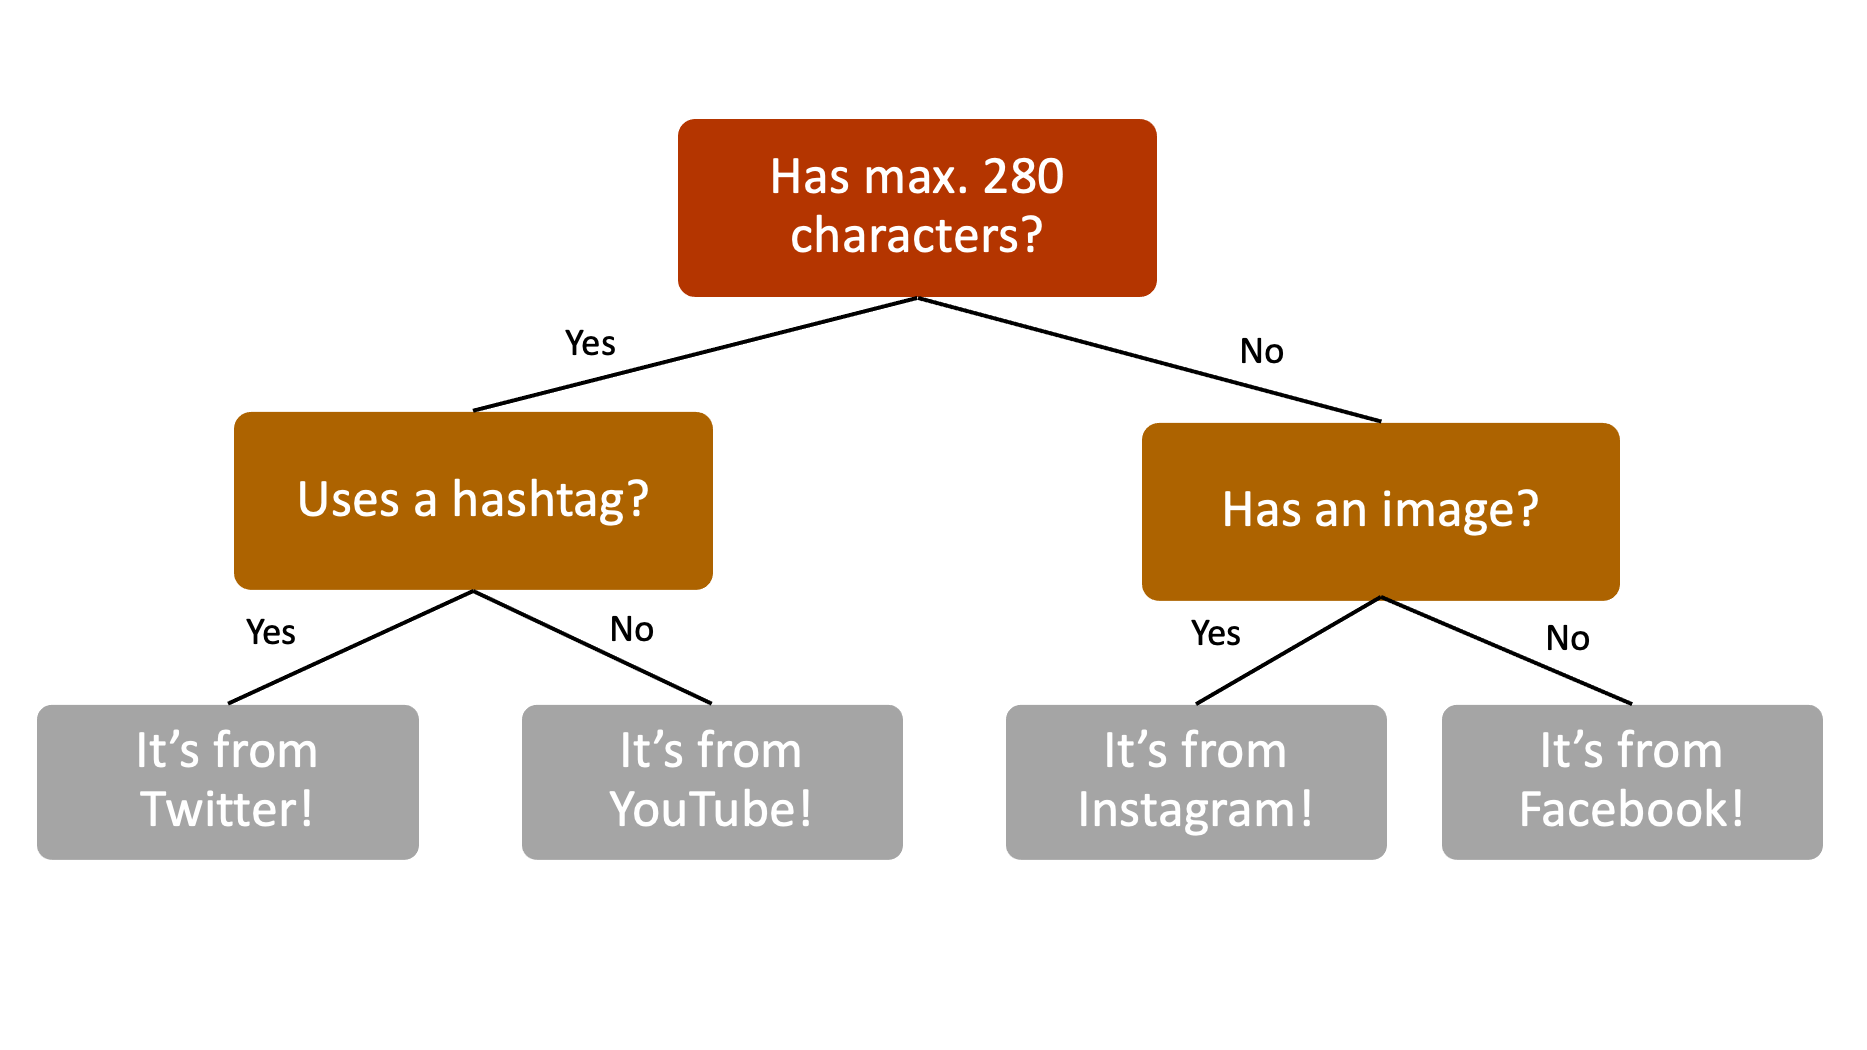
\includegraphics[width=\linewidth,height=\textheight,keepaspectratio]{../pictures/decisiontree.png} \\\
	\end{center}
	
	% In the previous sections, we discussed models that estimate linear relationships. So, we look at how an increase in an IV leads to a similar increase in the DV.
	
	% What about situations in which we want to know whether the value of a feature is above (or below) a specific threshold. For example, we want the computer to tell us the source of social media messages. 
	
	% Length is important here: If the message is longer than 280 characters, it cannot be from Twitter, for example. Note that this is the only thing we care about: whether a message is 281 characters long or 100.000 characters long doesn’t matter to us, we just want to know if it longer than 280 characters or not to be able to determine if Twitter is the source.
	
	% We can use a decision tree to learn more about this. This represents a stepwise decision process in which we first check one feature (i.e., the length) before checking another feature (e.g., presence of a hashtag).
	
	% Of course, this model will be wrong sometimes: some posts may be longer than 280 characters and contain an image but are posted on Facebook instead of Instagram, for example.
	
	% In Machine learning, the computer estimates this decision tree based on the data: it determines what features to look at and in what order to look at them.
	 
	
\end{frame}



\begin{frame}{Decision Trees and Random Forests} 
	
	Advantages of decision trees:
	\begin{itemize}
		\item Transparency
		\item Suitable for non-linear relationships \\\
	\end{itemize}
	
	Disadvatanges of decision trees:
	\begin{itemize}
		\item Loss of nuance due to yes/no-design
		\item Cannot correct early mistakes
		\item Prone to overfitting
	\end{itemize}


\end{frame}


\begin{frame}{Decision Trees and Random Forests}
	
	\begin{center}
		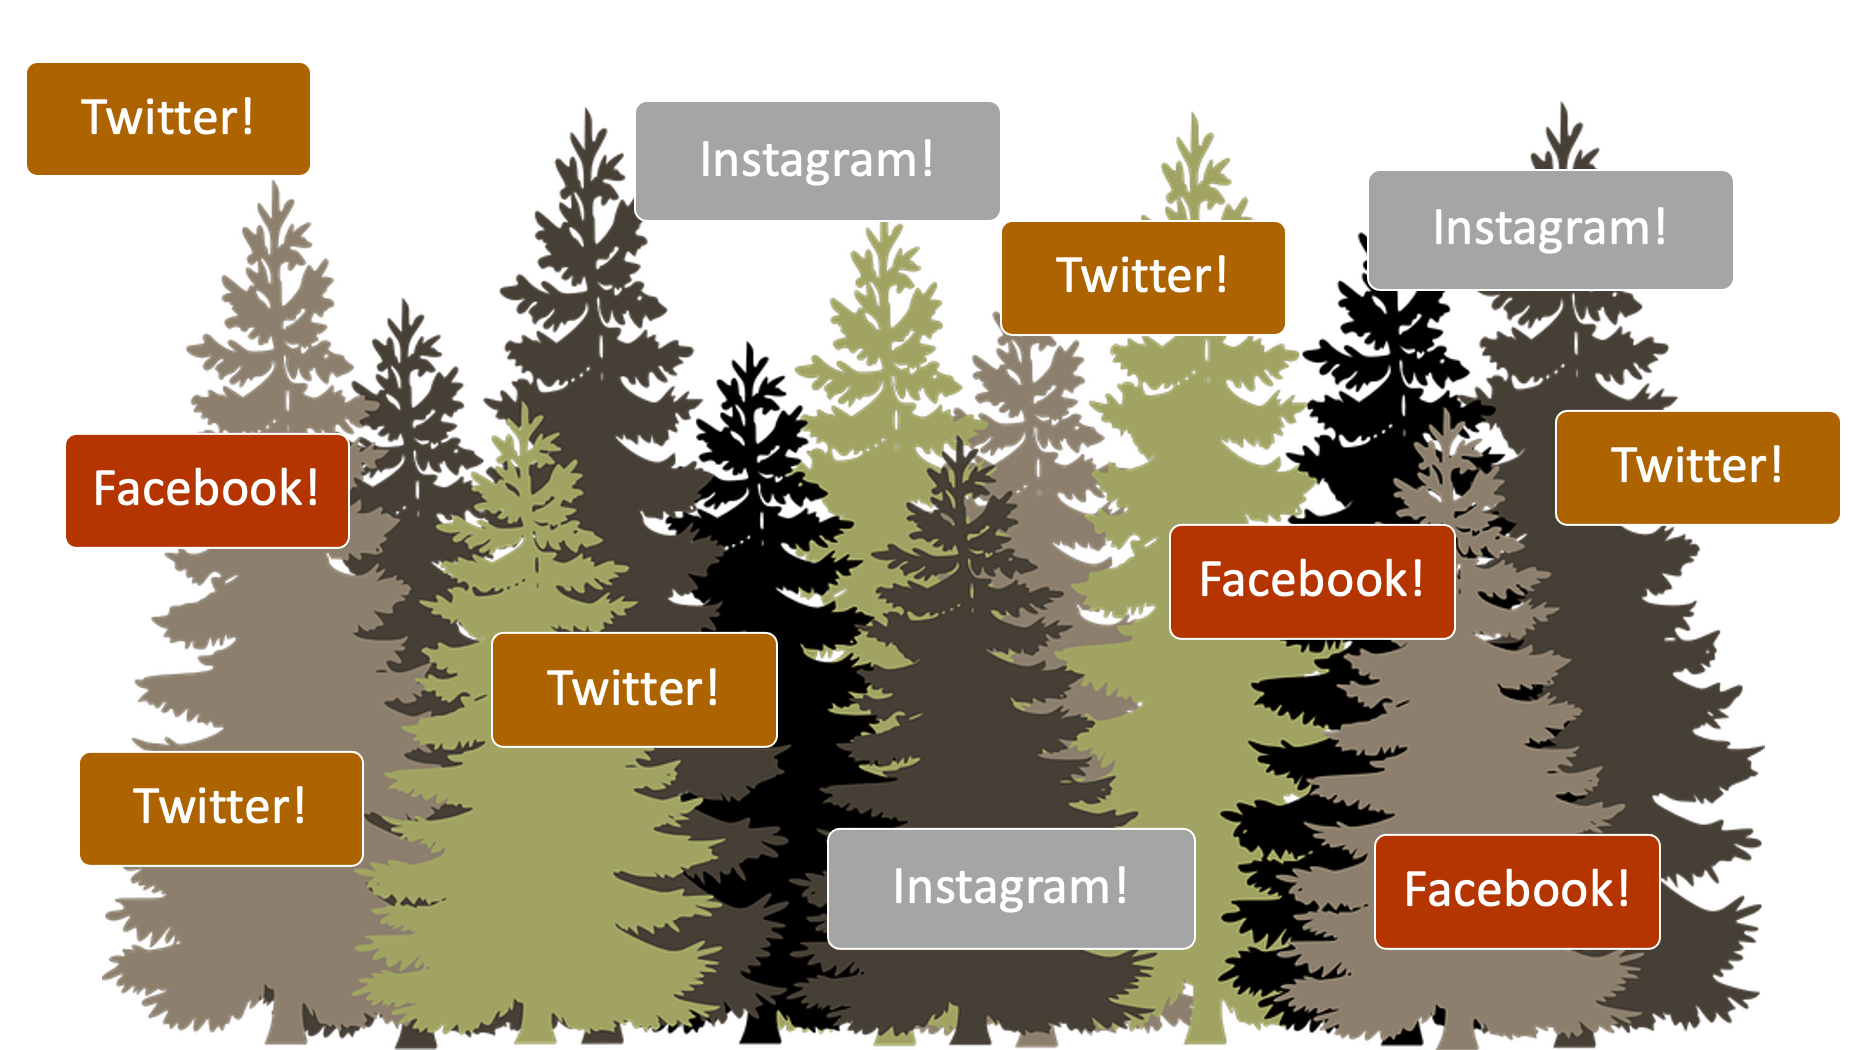
\includegraphics[width=\linewidth,height=\textheight,keepaspectratio]{../pictures/randomforest.png} \\\
	\end{center}
	
	% Solution to these disadvantages: Random forests! 

	% Drawing random samples from the data, multiple decision trees are estimated: we create a forest. We let each tree “vote” on what the outcome should be. This way, through majority voting, we come to a conclusion.

	% Using forests, we alleviate the problems of decision trees but we are still able to model non-linear relationships.
	
	% Connect to literature-example
	
\end{frame}


\begin{frame}{Neural Networks}
	
	\begin{center}
		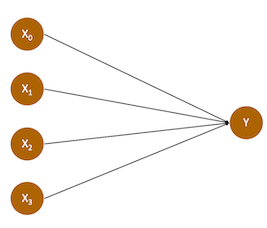
\includegraphics{../pictures/perceptron.png} \\\
	\end{center}
	
% What does a computer actually do with the models discussed above? In this lecture, we discuss neural networks as a machine learning algorithm.

% Neural networks consist of connection between neurons that are activated if the total input is above a certain threshold. Simplest form: perceptron.

% A perceptron is a single-layer neural network.

% Input neurons (or IV’s) connected to an output neuron (or DV). Each of the connections between neurons has a weight which can be positive or negative. For the output neuron, the weighted sum of inputs is calculated and a function is applied to determine the results. Which function is not set, it could be, for example, a logistic regression!

\end{frame}


\begin{frame}{Neural Networks}
	
	\begin{center}
		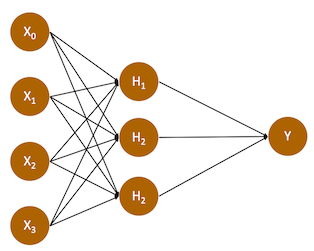
\includegraphics{../pictures/neuralnetwork_hiddenlayer.png} \\\
	\end{center}

	\begin{tiny}
	\fullcite{ha_automatically_2021} 
	\end{tiny}
	
% Imagine we use machine learning to determine the positivity or negativity of online movie reviews (sentiment analysis). The input neurons could be the frequencies of words such as “great” (positive weight) and “horrible” (negative weight). Such a network is a bit simplistic, because a review that says something is “not great” is negative but this wouldn’t be picked up by our network.

% To solve this, we can add a hidden layer of latent variables between the input and the output layer of the network.

% Connect to Ha et al. (link to deep learning)

	
\end{frame}


\begin{frame}{Recap}
	
	Many different models available for machine learning.
	
	How do you know what is the best for your case? Try it out and validate!
	
% We discussed only a few of the many available models for machine learning. Which model is best, depends on the characteristics of your project. Often, researchers run multiple models and then evaluate them to determine which one works best for them.
\end{frame}



\begin{frame}{Zooming out} 
	
	We talked about:
	\begin{itemize}
		\item The principles behind SML
		\item The steps of SML
		\item Some commonly used ML models \\\
	\end{itemize}
	
	Next, we will talk about:
	\begin{itemize}
		\item Validating models
	\end{itemize}
	
\end{frame}


\section{Validating models}


\begin{frame}{Precision and Recall}
	
	Precision quantifies the number of positive class predictions that actually belong to the positive cases. \\\ 
	OR: How much of what we found is actually correct?
	
	Recall quantifies the number of positive class prediction made out of all positive examples in the dataset. \\\
	OR: How many of the cases that we wanted to find did we actually find?

% Comment:
% Many different models that you can use! Which one is the best? Hard to say… often (as you could read for example, in Van Zoonen and Van der Meer for example) we try out different models and then we compare to determine which one is best. 

% To validate models, we use two measures: precision and recall.


\end{frame}
	


\begin{frame}{Precision and Recall}
	
	\begin{center}
		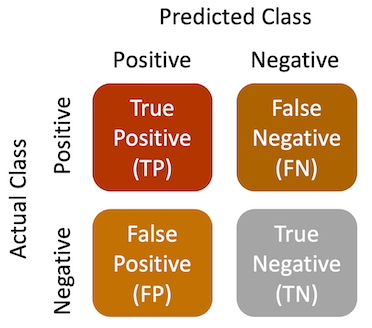
\includegraphics{../pictures/confusionmatrix_words.png} \\\
	\end{center}
	
% To estimate precision and recall, we can create a confusion matrix.

% This is a table where the columns represent the number of cases in a predicted class and the rows represent the number of cases in the real or actual class.

% Imagine we build a sentiment classifier of movie reviews. We want to find only movies that received good reviews. So, we have two goals: we want to receive as many good movies as possible (recall) and we also want to find only good movies (and not movies that got many bad reviews) (precision).

		
\end{frame}


\begin{frame}{Precision and Recall} 
	
	\begin{columns}
		\column{.3\textwidth}
		\makebox[\columnwidth]{
			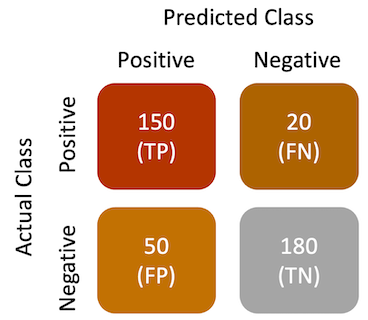
\includegraphics[width=\columnwidth,height=\paperheight,keepaspectratio]{../pictures/confusionmatrix_numbers.png}}
		\column{.7\textwidth}
		Precision is calculated as: \(\frac{\rm{TP}}{\rm{TP}+\rm{FP}}\) \\\
		In our case \(\frac{\rm{150}}{\rm{150}+\rm{50}}\) which is \(0.75\) \\\
		Recall is calculated as \(\frac{\rm{TP}}{\rm{TP}+\rm{FN}}\) \\\
		In our case \(\frac{\rm{150}}{\rm{150}+\rm{20}}\) which is \(0.88\)
	\end{columns}


% A not precise model may find a lot of the positives, but its selection method is noisy: it also wrongly detects many positives that aren’t actually positives.
% A precise model is very “pure”: maybe it does not find all the positives, but the ones that the model does class as positive are very likely to be correct

% A model with high recall succeeds well in finding all the positive cases in the data, even though they may also wrongly identify some negative cases as positive cases.
% A model with low recall is not able to find all (or a large part) of the positive cases in the data.

\end{frame}



\begin{frame}{Precision and Recall}
	
	\begin{center}
		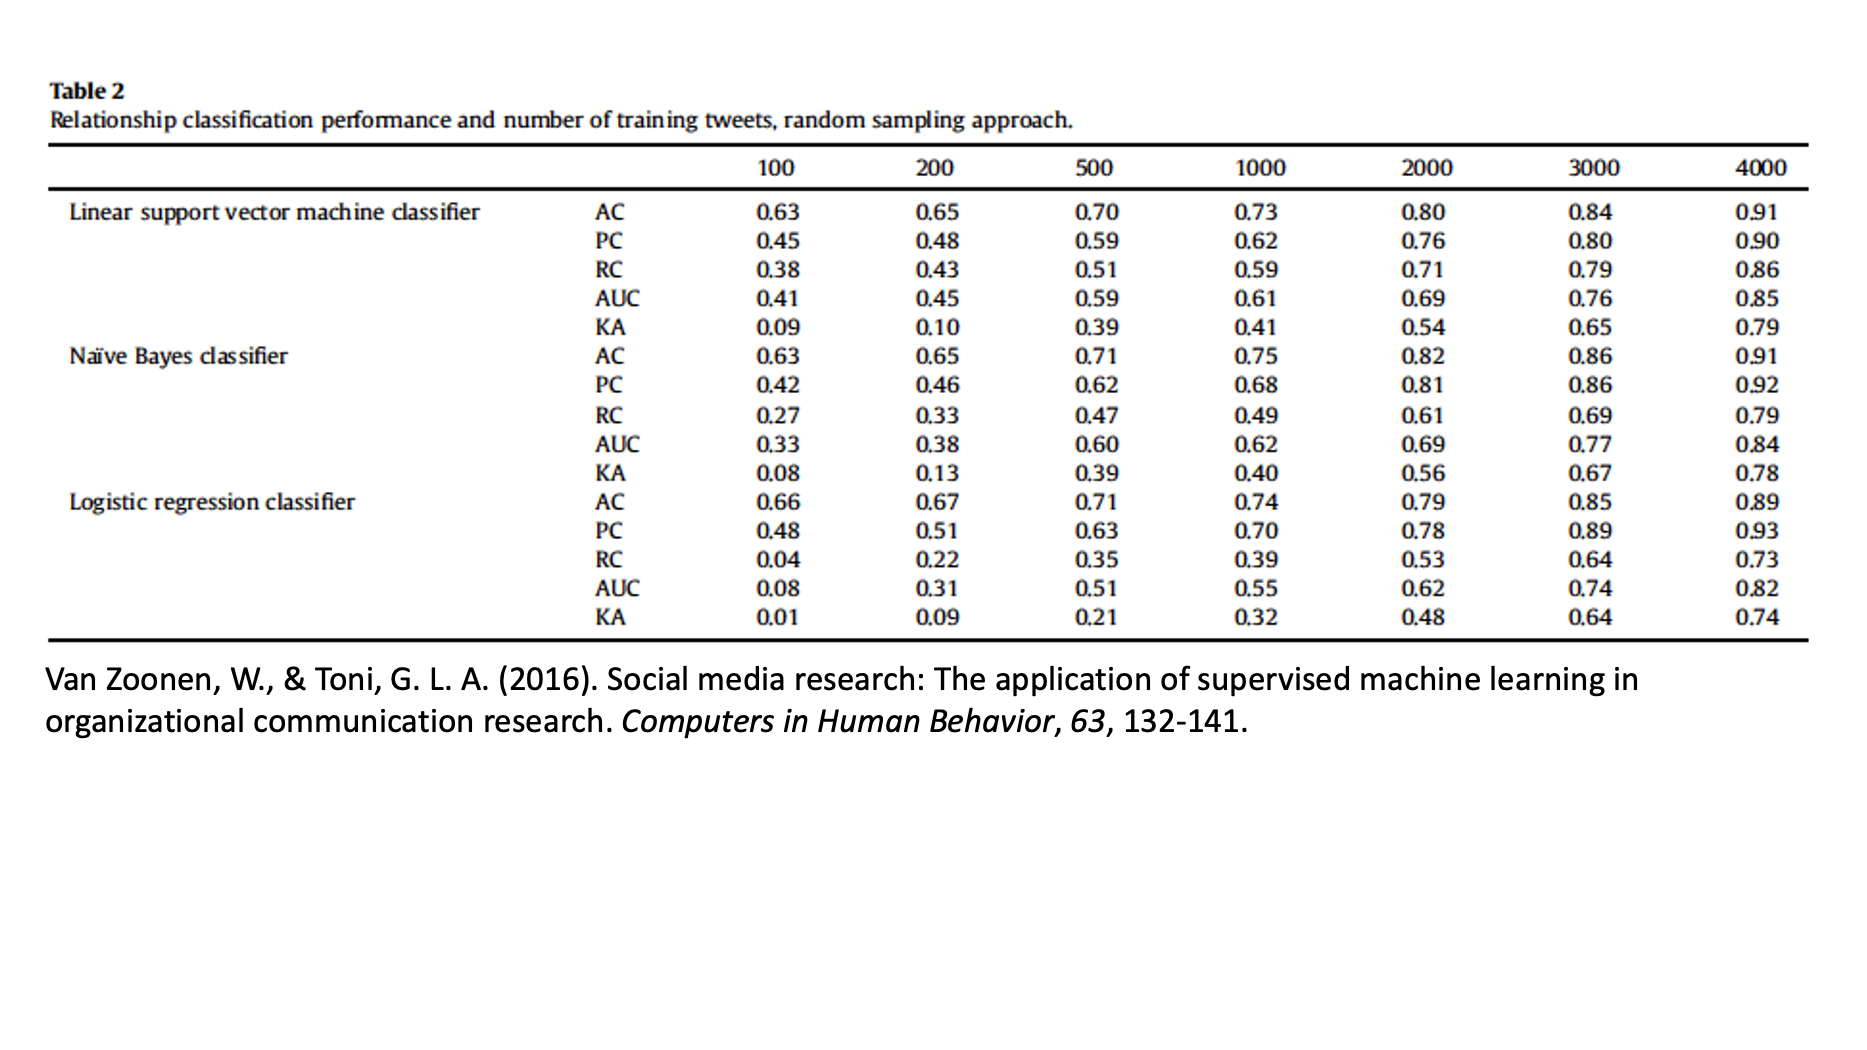
\includegraphics[width=\linewidth,height=\textheight,keepaspectratio]{../pictures/VanZoonen.png} \\\
	\end{center}

	\begin{tiny}
	\fullcite{van_zoonen_social_2016} 
	\end{tiny}

	
% Discuss example: Van Zoonen & Van der Meer (2016)

% As you read in this paper, there are more metrics in addition to precision and recall. 

\end{frame}


\begin{frame}{Accuracy}
	
		Accuracy: In which percentage of all cases was our classifier right? \\
		
		Class distribution: The number of examples that belong to each class. \\
		
		Imbalanced classification: A classification predictive modeling problem where the distribution of examples across the classes within a training dataset is not equal.
	
	% Slide about accuracy. Discuss class imbalance (https://machinelearningmastery.com/what-is-imbalanced-classification/)
	
\end{frame}


\begin{frame}{Accuracy}
	
	\begin{center}
		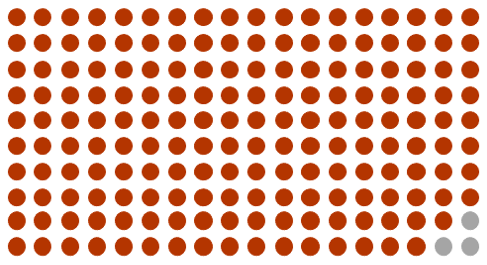
\includegraphics[width=\linewidth,height=\textheight,keepaspectratio]{../pictures/imbalance.png} 
	\end{center}	
	
	Majority class (red dots) vs. minority class (grey dots) 
	
	% Problem of imbalance remains to be solved
	% Some examples in which this is a problem: fraud detection, spam detection... and outlier detection
	
	%Linking back to accurcay: if we would label all dots as "red", we get a high accuracy score: we were right in almost all cases. But how valuable is this: we missed those crucial three cases that we wanted to learn more about!
	
	%More: https://machinelearningmastery.com/what-is-imbalanced-classification/	
\end{frame}



\begin{frame}{\(F_1\)-score}
	
	\(F_1\)-score: The harmonic mean of precision and recall. \\
	
	\(F_1\)-score \(= 2 \cdot \frac{\rm precision \cdot recall}{\rm precision + recall}\)

% Since the F1 score is an average of Precision and Recall, it means that the F1 score gives equal weight to Precision and Recall:
% A model will obtain a high F1 score if both Precision and Recall are high
% A model will obtain a low F1 score if both Precision and Recall are low
% A model will obtain a medium F1 score if one of Precision and Recall is low and the other is high

	
\end{frame}


\begin{frame}{Validating Models}
	
	Many more metrics to validate models. \\
	
	Learn more using, for example, the scikit-learn documentation. 
	
\end{frame}


\begin{frame}{Cross-validation}
	
	Overfitting: When a model fits \emph{exactly} against the data.
	
	When we calculate the metrics discussed above for multiple models on the same test dataset, we run the risk of overfitting on the test data.
	
	Potential solution: Split the dataset into three smaller sets. A training dataset, a validation dataset and a test dataset.
	
	However, this requires us to have a very large labeled dataset. In reality, this is not always the case!
	
	%Consequence of this is, for example, that your model can classify your training data perfectly, but it can't classify other data very well anymore.
	
	%Overfitting the model generally takes the form of making an overly complex model to explain idiosyncrasies in the data under study. In reality, the data often studied has some degree of error or random noise within it. Thus, attempting to make the model conform too closely to slightly inaccurate data can infect the model with substantial errors and reduce its predictive power.
	
\end{frame}


\begin{frame}{Cross-validation}
	
	Cross-validation: A resampling procedure to evaluate ML models on a limited data sample.
	
	\(k\)-fold cross-validation, where \(k\) refers to the number of groups or folds in which a sample is split.

\end{frame}


\begin{frame}{\(k\)-fold cross-validation}
	\(k\)-fold cross-validation step by step:
	\begin{enumerate}
		\item Shuffle the data
		\item Split the data into \(k\) folds (groups)
		\item For each unique group
		\begin{enumerate}
			\item Take the group as a test dataset
			\item Take the remaining groups as one training dataset
			\item Fit a model on the training set and evaluate it on the test set
			\item Retain the evaluation score and discard the model
		\end{enumerate}
		\item Summarize the evaluation scores to assess the model \\\
	\end{enumerate}

\end{frame}
	

\begin{frame}{Cross-validation}
	
	Cross-validation is often used to compare many different model specifications, for example to find the best hyperparameters.
	
	Hyperparameters: Parameters of the model that are not estimated from the data. 
	
	To do this, the Grid Search algorithm is often used.
	
	More about hyperparameters in this week's tutorial!
	
\end{frame}




\begin{frame}{Zooming out} 
	
	We talked about:
	\begin{itemize}
		\item The principles behind SML
		\item The steps of SML
		\item Some commonly used ML models
		\item Validating models \\\
	\end{itemize}
	
	Next, we will talk about:
	\begin{itemize}
		\item Strengths and challenges associated to SML
	\end{itemize}
	
\end{frame}


\section{SML: Strenghts and Challenges}


\begin{frame}{Strengths and Challenges} 
	
	Strengths:
	\begin{itemize}
		\item Easier to code large datasets
		\item Enhances replicable research
		\item Easier to study "natural" human behavior \\\
	\end{itemize}
	
	Disadvantages:
	\begin{itemize}
		\item Resource constraints
		\item Ethical considerations
		\item Criticism required (see next slide)
	\end{itemize}

% Strengths:
% -	Makes it easier to code large datasets (cheaper, faster)
% -	Enhances replicable research (exactly the same script can be used to by researchers to conduct a new content analysis)
% -	Makes it easier to study “natural” human behavior (example: study social influence by hiring actors to see if it influences people’s reactions to videos; now, we can just analyze the comments people write and how these influence subsequent comments!)

% Challenges
% -	(Jordan & Mitchell, p. 5) Resource constraint (privacy, required processing capacities  communication constraint
% -	Ethical questions: Who will have access to, and ownership of, online data and who will reap its benefits? (Jordan & Mitchell, p.6)

\end{frame}


\begin{frame}{Strengths and Challenges}
	
	\begin{center}
		
\includegraphics[width=\linewidth,height=\textheight,keepaspectratio]{../pictures/toeslagenaffaire_headlines.png} \\\
	\end{center}
	
% As shown by Jordan & Mitchell, ML is used in many different facets of society. But it is impertinent that those who use ML remain critical of its capabilities. If a machine is trained based on human coded data, as is the case with SML, it will also learn about the prejudices that humans have: toeslagenaffaire voorbeeld. Laag inkomen werd door computer geleerd als voorspeller van fraude. Mensen met een laag inkomen werden er dus bij voorbaat al uitgepikt. 
%  Remember that in the end, machines are created by humans and as humans we are responsible for how we use them. We have the responsibility to ask questions about what machines do and how and whether we should!
	
\end{frame}


\begin{frame}{Zooming out I} 
	
	We talked about:
	\begin{itemize}
		\item The principles behind SML
		\item The steps of SML
		\item Some commonly used ML models
		\item Validating models
		\item Strengths and challenges associated to SML \\\
	\end{itemize}
	
	
\end{frame}

\begin{frame}{Zooming out II} 
	
	This week's tutorial:
	\begin{itemize}
		\item Hands-on approach to take a further look into the machine learning process
		\item Tutorial goals:
		\begin{itemize}
			\item To get you some experience with the SML process and selecting a model
			\item To provide a stepping stone so that you can (independently) advance your machine learning skills
		\end{itemize}
		
	\end{itemize}
	
\end{frame}


\end{document}